% #####################################################################
% #####################################################################
% ##                                                                 ##
% ##                             Lizenz:                             ##
% ##                         CC BY-NC-SA 3.0                         ##
% ##      http://creativecommons.org/licenses/by-nc-sa/3.0/de/       ##
% ##                                                                 ##
% #####################################################################
% ##   Diese Datei kann beliebig verändert werden, solange darauf    ##
% ##     hingewiesen wird, dass dieses Dokument ursprünglich von     ##
% ##                                                                 ##
% ##                        www.ei-studium.de                        ##
% ##                                                                 ##
% ##                             stammt.                             ##
% ## Dies gilt insbesondere auch für alle daraus erstellten Dateien. ##
% ##    Des Weiteren muss die Weitergabe dieser Dateien unter der    ##
% ##                    gleichen Lizenz erfolgen.                    ##
% #####################################################################
% #####################################################################
\documentclass[a4paper,twocolumn,10pt]{article}
\usepackage[utf8]{inputenc}
\usepackage[ngerman]{babel}
\usepackage[top=2.0cm,bottom=1.5cm,left=1.0cm,right=1.0cm]{geometry}
\usepackage{enumitem}
\usepackage{graphicx}
\usepackage{amsfonts}
\usepackage{amsmath}
\usepackage{sectsty}
\usepackage{colortbl}
\usepackage{cancel}
\usepackage{listings}
\usepackage{color}
\usepackage{amsmath}
\usepackage{fancyhdr}
% for highlighting with \hl{}
\usepackage{soul}
\setlist{itemsep=.01mm}
\setenumerate{label=\emph{\arabic*})}
\setlength{\columnsep}{1cm}
\parindent 0mm

\partfont{\huge}
\sectionfont{\Large \sc\bf}
\subsectionfont{\normalsize}
\subsubsectionfont{\small\textit}

\pagestyle{fancy}
\lhead[\leftmark]{Schaltungstechnik 2}
\chead[\leftmark]{TEAM INFORMATIK (Vorlage von www.ei-studium.de)}
\rhead[\leftmark]{Erstelldatum: \today}
\lfoot[\leftmark]{Keine Garantie auf Vollständigkeit und Richtigkeit!}
\cfoot[\leftmark]{}
\rfoot[\leftmark]{\thepage}
\renewcommand{\headrulewidth}{0.5pt}
\renewcommand{\footrulewidth}{0.5pt}

\newcommand{\entspr}{\widehat{=}}
\newcommand{\sollsein}{\stackrel{!}{=}}

\begin{document}

\part*{Schaltungstechnik 2}

\section*{Reaktive Netzwerkelemente}

\begin{minipage}[t]{0.23\textwidth}
\subsection*{Kapazität}
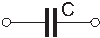
\includegraphics[width=0.5\textwidth]{img/Kapazitaet}
\end{minipage}
\hfill
\begin{minipage}[t]{0.23\textwidth}
\subsection*{Induktivität}
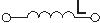
\includegraphics[width=0.5\textwidth]{img/Induktivitaet}
\end{minipage}

\subsubsection*{Allgemein}
\begin{minipage}[b]{0.23\textwidth}
$[C]=\frac{As}{V}=F$\\\\
Ladung $q: [q]=As=C$\\\\
$i(t) = \frac{dq(t)}{dt}= \dot q(t)$\\\\
$q(t)=q_0+\int\limits_{t_0}^{t}i(\tau)d\tau$\\\\
$C=\frac{dq}{du}$
\end{minipage}
\hfill
\begin{minipage}[b]{0.23\textwidth}
$[L]=\frac{Vs}{A}=H$\\\\
Fluss $\Phi: [\Phi]=Vs=Wb$\\\\
$u(t) = \frac{d\Phi(t)}{dt}= \dot \Phi(t)$\\\\
$\Phi(t)=\Phi_0+\int\limits_{t_0}^{t}u(\tau)d\tau$\\\\
$L=\frac{d\Phi}{di}$
\end{minipage}

\subsubsection*{Lineare Reaktanz}
\begin{minipage}[b]{0.23\textwidth}
$q(t)=C \cdot u(t)$\\\\
$i(t)=C \cdot \dot u(t)$
\end{minipage}
\hfill
\begin{minipage}[b]{0.23\textwidth}
$\Phi (t)=L\cdot i(t)$\\\\
$u(t)=L\cdot \dot i(t)$
\end{minipage}

\subsubsection*{Blindwiderstand}
\begin{minipage}[b]{0.23\textwidth}
$X_C=\frac{1}{\omega C}$
\end{minipage}
\hfill
\begin{minipage}[b]{0.23\textwidth}
$X_L=\omega L$
\end{minipage}

\subsection*{Zusammenschaltung reaktiver Eintore}
\subsubsection*{Kapazität}
\begin{tabular}{ll}
Reihenschaltung: & $\frac{1}{C_{gesamt}}=\frac{1}{C_1}+...+\frac{1}{C_i}$\\\\
Parallelschaltung: & $C_{gesamt}=C_1+...+C_i$

\end{tabular}

\subsubsection*{Induktivität}
\begin{tabular}{ll}
Reihenschaltung: & $L_{gesamt}=L_1+...+L_i$\\\\
Parallelschaltung: & $\frac{1}{L_{gesamt}}=\frac{1}{L_1}+...+\frac{1}{L_i}$\\\\
\end{tabular}

\subsection*{Dualität}
$(u,q)\in F \Leftrightarrow (\frac{u}{R_d},R_dq)=(i,\Phi)\in F^d$\\\\
$(i,\Phi)\in F \Leftrightarrow (R_di,\frac{\Phi}{R_d})=(u,q)\in F^d$\\\\
$C=\frac{L}{R_d^2};\;\;\;\;\;L=C\cdot R_d^2$

\subsection*{Eigenschaften}
\begin{tabular}{ll}
\textbf{$F$ ist...} & \textbf{Kennlinie von $F$...}\\
- kapazitiv & $\exists $ Beziehung zwischen $q$ und $u$\\
- induktiv & $\exists $ Beziehung zwischen $\Phi$ und $i$\\
- ungepolt & ... ist punktsymmetrisch zu $(0,0)$\\
- spannungsgesteuert & $\exists$ Darstellung $q=c(u)$\\
- stromgesteuert & $\exists$ Darstellung $\Phi=l(i)$\\
- ladungsgesteuert & $\exists$ Darstellung $u=c^{-1}(q)$\\
- flussgesteuert & $\exists$ Darstellung $i=l^{-1}(\Phi)$\\
- streng linear & ... ist Ursprungsgerade, Ursprung\\
 & \;\;\;\;oder ganze $u$-$q$- bzw. $i$-$\Phi$-Ebene\\
- linear & ... ist eine beliebige Gerade\\
- stückweise linear & ... besteht aus Geradenstücken\\
- verlustfrei & ... liegt vollständig auf den Achsen der\\
              & ~~~u-i. - Ebene $\forall t. p(t)=u(t)i(t)=0$
\end{tabular}

\subsection*{Netzwerkelemente mit Mehrfachcharakter}
\begin{enumerate}[label=-,leftmargin=3mm]
	\item Nullator, Norator, Leerlauf und Kurzschluss sind resistiv, kapazitiv, induktiv und memristiv
	\item Spannungsquellen sind resistiv und kapazitiv
	\item Stromquellen sind resistiv und induktiv
\end{enumerate}

\subsection*{Energie}
Ideale Reaktanzen sind verlustlos, falls die Kennlinie keine geschlossenen Schleifen enthält.

\subsubsection*{Kapazität}
$W_C=\int\limits_{t_1}^{t_2}u(t)\cdot i(t)dt= \int\limits_{t_1}^{t_2}u(t)\cdot \frac{dq(t)}{dt}dt = \int\limits_{q_1}^{q_2}u(q)dq$\\\\\\
Falls linear: $W_C=\frac{C}{2}\cdot u^2=\frac{1}{2C}\cdot q^2$

\subsubsection*{Induktivität}
$W_L=\int\limits_{t_1}^{t_2}u(t)\cdot i(t)dt= \int\limits_{t_1}^{t_2}i(t)\cdot \frac{d\Phi(t)}{dt}dt = \int\limits_{\Phi_1}^{\Phi_2}i(\Phi)d\Phi$\\\\\\
Falls linear: $W_L=\frac{L}{2}\cdot i^2=\frac{1}{2L}\cdot \Phi^2$

\subsubsection*{Relaxationspunkte}
Relaxationspunkte (=Ruhepunkte):\\
Betriebspunkt, in dem die in einer Reaktanz gespeicherte Energie minimal ist.\\
Um zu einem anderen Punkt zu gelangen, muss stets Energie aufgenommen werden.\\\\
Kandidaten:\\
Extremwerte, Wendepunkte, Knicke, Schnittpunkte mit Achsen\\\\
Energie steigt falls:\\
$u>0 \land q$ steigt \underline{oder} $u<0 \land q$ fällt.\\
bzw.\\
$i>0 \land \Phi$ steigt \underline{oder} $i<0 \land \Phi$ fällt.\\\\
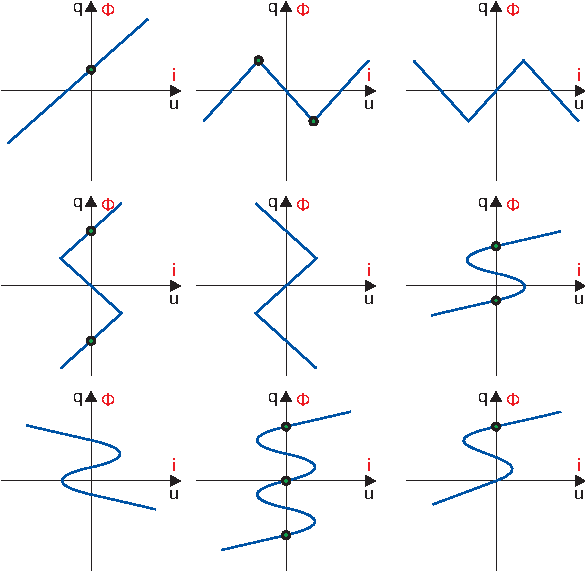
\includegraphics[width=0.45\textwidth]{img/Relaxationspunkte}

\section*{Schaltungen ersten Grades}
\subsection*{1. Ersatzschaltbild erstellen}
\begin{minipage}[t]{0.23\textwidth}
\subsubsection*{Kapazität}
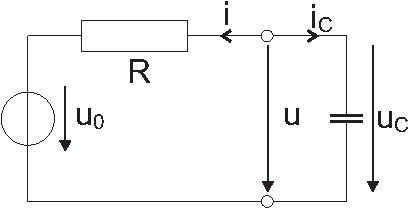
\includegraphics[width=0.95\textwidth]{img/Helmholz-Thevenin}\\
Helmholz / Thevenin\\\\
Zustandsgröße: $u_c(t)$\\\\
Zeitkonstante: \hl{$\tau = R\cdot C$}
\end{minipage}
\hfill
\begin{minipage}[t]{0.23\textwidth}
\subsubsection*{Induktivität}
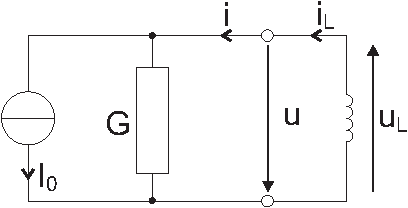
\includegraphics[width=0.95\textwidth]{img/Mayer-Norton}\\
Mayer / Norton\\\\
Zustandsgröße: $i_L(t)$\\\\
Zeitkonstante: \hl{$\tau = G\cdot L$}
\end{minipage}

\subsection*{2. Differentialgleichung aufstellen}
\begin{minipage}[t]{0.23\textwidth}
$i_c(t)=C\cdot \dot u_c(t)$\\\\
$i(t)=\frac{u_c-U_0}{R}$\\\\
$C\cdot \dot u_c(t)=-\frac{u_c-U_0}{R}$\\\\
\underline{$\dot u_c=-\frac{1}{RC}\cdot u_c+\frac{1}{RC}\cdot U_0$}
\end{minipage}
\hfill
\begin{minipage}[t]{0.23\textwidth}
$u_L(t)=L\cdot \dot i_L(t)$\\\\
$u(t)=\frac{i_L-I_0}{G}$\\\\
$L\cdot \dot i_L(t)=-\frac{i_L-I_0}{G}$\\\\
\underline{$\dot i_L=-\frac{1}{GL}\cdot i_L+\frac{1}{GL}\cdot I_0$}
\end{minipage}

\subsection*{3. Lösung der Differentialgleichung}
\subsubsection*{Konstante Erregung}
Kapazität:\\\\
\underline{$u_c(t)=u_C(t_{\infty})+[u_C(t_0)-u_C(t_{\infty})]\cdot e^{\frac{t_0-t}{\tau}}$}\\\\
$i_C(t)=-\frac{C}{\tau}[u_C(t_0)-u_C(t_{\infty})]\cdot e^{\frac{t_0-t}{\tau}}$\\\\
$u_C(t_{\infty})= U_0\;\;\;(\dot u_C\sollsein 0)$ Gleichgewichtszustand\\\\
Induktivität:\\\\
\underline{$i_L(t)=i_L(t_{\infty})+[i_L(t_0)-i_L(t_{\infty})]\cdot e^{\frac{t_0-t}{\tau}}$}\\\\
$u_L(t)=-\frac{L}{\tau}[i_L(t_0)-i_L(t_{\infty})]\cdot e^{\frac{t_0-t}{\tau}}$\\\\
$i_L(t_{\infty})= I_0\;\;\;(\dot i_L\sollsein 0)$ Gleichgewichtszustand

\subsubsection*{Abschnittsweise konstante Erregung}
Vorgehensweise wie zuvor, jedoch muss die Berechnung in Intervalle aufgeteilt werden.\\
Für jedes Intervall muss der Startwert berechnet werden.

\subsubsection*{Allgemeine Erregung}
$u_C(t)=\underbrace{u_C(t_0)\cdot e^{\frac{t_0-t}{\tau}}}_{zero\;input\;response}+\underbrace{\int\limits_{t_0}^{t}\frac{1}{\tau}\cdot u_0(t')\cdot e^{\frac{t'-t}{\tau}}dt'}_{zero\;state\;response}\; \forall t \geq t_0$\\\\
$i_L(t)=i_L(t_0)\cdot e^{\frac{t_0-t}{\tau}}+\int\limits_{t_0}^{t}\frac{1}{\tau}\cdot i_0(t')\cdot e^{\frac{t'-t}{\tau}}dt'$

\subsection*{Kurvenverlauf}
\begin{enumerate}[label=-,leftmargin=3mm]
	\item Kapazität: $u_C$ ist stetig; $i_C$ kann springen
	\item Induktivität: $i_L$ ist stetig; $u_L$ kann springen
\end{enumerate}

\subsubsection*{Stabiler Fall: $\tau>0$}
\begin{enumerate}[label=-,leftmargin=3mm]
	\item Tangente an Kurve in ($t_0,x_0$) verläuft durch ($t_0+\tau,x_\infty$)
	\item Kurve hat sich nach $1\tau$ um $0,63\cdot |x_0-x_\infty|$ in Richtung $x_\infty$ bewegt
	\item Nach $7\tau$ ist $x_\infty$ praktisch erreicht
\end{enumerate}
\begin{minipage}[t]{0.23\textwidth}
$x_\infty > x_0$\\\\
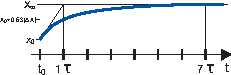
\includegraphics[width=0.98\textwidth]{img/Zeitverlauf1}\\
\end{minipage}
\hfill
\begin{minipage}[t]{0.23\textwidth}
$x_\infty < x_0$\\\\
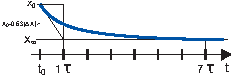
\includegraphics[width=0.98\textwidth]{img/Zeitverlauf2}\\
\end{minipage}

\subsubsection*{Instabiler Fall: $\tau<0$}
\begin{enumerate}[label=-,leftmargin=3mm]
	\item Tangente an Kurve in ($t_0,x_0$) verläuft durch ($t_0+\tau,x_0\pm |x_0-x_\infty|$) bzw. durch ($t_0-|\tau|,x_\infty$)
	\item Kurve hat sich nach $1\tau$ um $1,72\cdot |x_0-x_\infty|$ entgegen der Richtung $x_\infty$ bewegt
	\item Kurve geht gegen $\pm \infty$
	\item $\lim\limits_{t\rightarrow -\infty} x(t)=x_\infty$
	\item Für eine negativ ablaufende Zeit wird $x_\infty$ praktisch nach $|7\tau|$ erreicht
\end{enumerate}
\begin{minipage}[t]{0.23\textwidth}
$x_\infty > x_0$\\\\
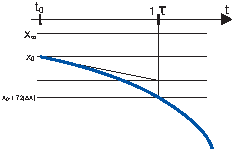
\includegraphics[width=0.98\textwidth]{img/Zeitverlauf3}\\
\end{minipage}
\hfill
\begin{minipage}[t]{0.23\textwidth}
$x_\infty < x_0$\\\\
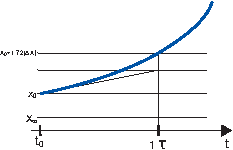
\includegraphics[width=0.98\textwidth]{img/Zeitverlauf4}\\
\end{minipage}

\subsection*{Abschnittsweise lineare Schaltungen}
\begin{minipage}[t]{0.23\textwidth}
Kapazitiv\\\\
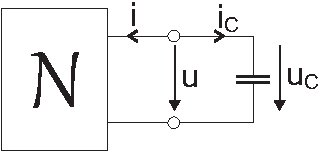
\includegraphics[width=0.98\textwidth]{img/DynamischerPfadN1}\\\\
$i=-C\cdot\dot u$
\end{minipage}
\hfill
\begin{minipage}[t]{0.23\textwidth}
Induktiv\\\\
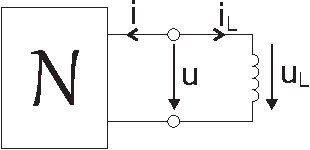
\includegraphics[width=0.98\textwidth]{img/DynamischerPfadN2}\\\\
$u=-L\cdot\dot i$
\end{minipage}
\subsubsection*{Dynamischer Pfad}
Anfangspunkt entspricht $u_C(t_0)$ bzw. $i_L(t_0)$\\\\
\underline{Pfadverlauf (Richtung):}\\\\
\begin{minipage}[t]{0.23\textwidth}
\underline{$i<0$} $\Rightarrow \dot u>0$\\
$\Rightarrow u$ muss zunehmen\\\\
\underline{$i>0$} $\Rightarrow \dot u<0$\\
$\Rightarrow u$ muss abnehmen
\end{minipage}
\hfill
\begin{minipage}[t]{0.23\textwidth}
\underline{$u<0$} $\Rightarrow \dot i>0$\\
$\Rightarrow i$ muss zunehmen\\\\
\underline{$u>0$} $\Rightarrow \dot i<0$\\
$\Rightarrow i$ muss abnehmen
\end{minipage}\\\\\\
\underline{Gleichgewichtspunkt (GGP):}\\\\
\begin{minipage}[t]{0.23\textwidth}
$\dot u_C=0 \Rightarrow i=0$
\end{minipage}
\hfill
\begin{minipage}[t]{0.23\textwidth}
$\dot i_L=0 \Rightarrow u=0$
\end{minipage}\\\\\\
Bei stabilen RC-Schaltungen endet der dynamische Pfad stets auf der $u$-Achse ($i_C=0$), bei stabilen RL-Schaltungen stets auf der $i$-Achse ($u_L=0$)\\\\
\underline{Tote Punkte:}\\\\
= Punkte, die keine Gleichgewichtspunkte sind und an denen der Pfad nicht entlang der Kennlinie fortgesetzt werden kann
($\Rightarrow$ Sprungphänomen)
\subsubsection*{Sprungphänomene}
Dauerhafte Sprungphänomene treten nur auf, falls der Gleichgewichtszustand nicht erreicht werden kann\\
($\Rightarrow$ Relaxationsoszillator, astabiler Multivibrator)\\\\
\begin{minipage}[t]{0.23\textwidth}
Kapazitiv\\
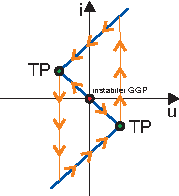
\includegraphics[width=0.98\textwidth]{img/PfadSprung1}\\\\
\end{minipage}
\hfill
\begin{minipage}[t]{0.23\textwidth}
Induktiv\\
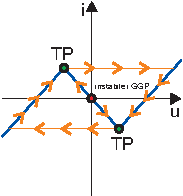
\includegraphics[width=0.98\textwidth]{img/PfadSprung2}\\\\
\end{minipage}\\\\
Vertauscht man bei der astabilen Multivibratorschaltung die ,,+'' und ,,-'' Klemmen des Op-Amp-Eingangstores, so erhält man eine bistabile Kippstufe (Flip-Flop), die durch eine Strom- bzw. Spannungsquelle getriggert werden kann

\section*{Lineare Schaltungen zweiten Grades}
\subsection*{Zustandsgleichung}
$\underline{\dot x}=\textbf{A}\cdot \underline{x}+\textbf{B}\cdot \underline{v}$\\\\
Zustandsvektor $\underline{x}\in \mathbb{R}^{2}$; Zustandsmatrix $\textbf{A}\in \mathbb{R}^{2\times 2}$\\
Einkoppelmatrix $\textbf{B}\in \mathbb{R}^{2\times k}$; Erregunsvektor $\underline{v}\in \mathbb{R}^{k}$\\
$k$: Anzahl der Erregungssignale
\subsection*{Ausgangsgleichung}
$\underline{y}=\textbf{C}\cdot \underline{x}+\textbf{D}\cdot \underline{v}$\\\\
$\underline{y}\in \mathbb{R}^{j}$; Auskoppelmatrix $\textbf{C}\in \mathbb{R}^{j\times 2}$; Durchgriff der Erregung $\textbf{D}\in \mathbb{R}^{j\times k}$; $j$: Anzahl der Ausgangssignale
\subsection*{1. ESB erstellen + Zweitorbeschreibung ermitteln}
\begin{minipage}[t]{0.23\textwidth}
\subsubsection*{Leitwertsbeschreibung}
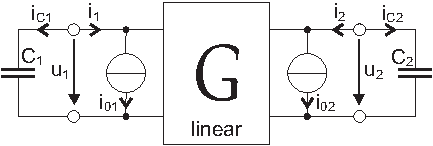
\includegraphics[width=0.98\textwidth]{img/ESBzweitenGrades1}\\\\
$\left.\begin{matrix}i_1 \\ i_2\end{matrix}\right]=\textbf{G}\cdot \underbrace{\left.\begin{matrix}u_1 \\ u_2\end{matrix}\right]}_{\underline{x}}+\left.\begin{matrix}i_{01} \\ i_{02}\end{matrix}\right]$
\end{minipage}
\hfill
\begin{minipage}[t]{0.23\textwidth}
\subsubsection*{Widerstandsbeschreibung}
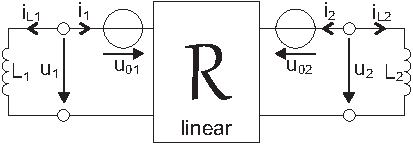
\includegraphics[width=0.98\textwidth]{img/ESBzweitenGrades2}\\\\
$\left.\begin{matrix}u_1 \\ u_2\end{matrix}\right]=\textbf{R}\cdot \underbrace{\left.\begin{matrix}i_1 \\ i_2\end{matrix}\right]}_{\underline{x}}+\left.\begin{matrix}u_{01} \\ u_{02}\end{matrix}\right]$
\end{minipage}\\\\\\
\begin{minipage}[t]{0.23\textwidth}
\subsubsection*{Hybridbeschreibung}
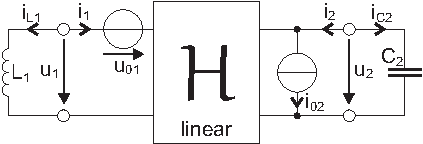
\includegraphics[width=0.98\textwidth]{img/ESBzweitenGrades3}\\\\
$\left.\begin{matrix}u_1 \\ i_2\end{matrix}\right]=\textbf{H}\cdot \underbrace{\left.\begin{matrix}i_1 \\ u_2\end{matrix}\right]}_{\underline{x}}+\left.\begin{matrix}u_{01} \\ i_{02}\end{matrix}\right]$
\end{minipage}
\hfill
\begin{minipage}[t]{0.23\textwidth}
\subsubsection*{Inverse Hybridbeschreibung}
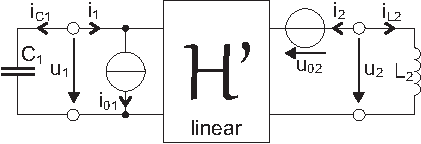
\includegraphics[width=0.98\textwidth]{img/ESBzweitenGrades4}\\\\
$\left.\begin{matrix}i_1 \\ u_2\end{matrix}\right]=\textbf{H'}\cdot \underbrace{\left.\begin{matrix}u_1 \\ i_2\end{matrix}\right]}_{\underline{x}}+\left.\begin{matrix}i_{01} \\ u_{02}\end{matrix}\right]$
\end{minipage}

\subsection*{2. Differentialgleichung aufstellen}
\begin{minipage}[t]{0.23\textwidth}
\subsubsection*{Leitwertsbeschreibung}
$\left.\begin{matrix}i_1 \\ i_2\end{matrix}\right]=\left.\begin{matrix}-C_1\cdot \dot u_1 \\ -C_2\cdot \dot u_2\end{matrix}\right]$\\\\
$\left.\begin{matrix}i_1 \\ i_2\end{matrix}\right]=\begin{bmatrix}-C_1 & 0 \\ 0 & -C_2\end{bmatrix}\cdot \underbrace{\left.\begin{matrix}\dot u_1 \\ \dot u_2\end{matrix}\right]}_{\underline{\dot x}}$
\end{minipage}
\hfill
\begin{minipage}[t]{0.23\textwidth}
\subsubsection*{Widerstandsbeschreibung}
$\left.\begin{matrix}u_1 \\ u_2\end{matrix}\right]=\left.\begin{matrix}-L_1\cdot \dot i_1 \\ -L_2\cdot \dot i_2\end{matrix}\right]$\\\\
$\left.\begin{matrix}u_1 \\ u_2\end{matrix}\right]=\begin{bmatrix}-L_1 & 0 \\ 0 & -L_2\end{bmatrix}\cdot \underbrace{\left.\begin{matrix}\dot i_1 \\ \dot i_2\end{matrix}\right]}_{\underline{\dot x}}$
\end{minipage}\\\\\\
\begin{minipage}[t]{0.23\textwidth}
\subsubsection*{Hybridbeschreibung}
$\left.\begin{matrix}u_1 \\ i_2\end{matrix}\right]=\left.\begin{matrix}-L_1\cdot \dot i_1 \\ -C_2\cdot \dot u_2\end{matrix}\right]$\\\\
$\left.\begin{matrix}u_1 \\ i_2\end{matrix}\right]=\begin{bmatrix}-L_1 & 0 \\ 0 & -C_2\end{bmatrix}\cdot \underbrace{\left.\begin{matrix}\dot i_1 \\ \dot u_2\end{matrix}\right]}_{\underline{\dot x}}$
\end{minipage}
\hfill
\begin{minipage}[t]{0.23\textwidth}
\subsubsection*{Inverse Hybridbeschreibung}
$\left.\begin{matrix}i_1 \\ u_2\end{matrix}\right]=\left.\begin{matrix}-C_1\cdot \dot u_1 \\ -L_2\cdot \dot i_2\end{matrix}\right]$\\\\
$\left.\begin{matrix}i_1 \\ u_2\end{matrix}\right]=\begin{bmatrix}-C_1 & 0 \\ 0 & -L_2\end{bmatrix}\cdot \underbrace{\left.\begin{matrix}\dot u_1 \\ \dot i_2\end{matrix}\right]}_{\underline{\dot x}}$
\end{minipage}
\subsection*{3. Gleichsetzen und Umformen}
\subsubsection*{Leitwertsbeschreibung}
$\begin{bmatrix}-C_1 & 0 \\ 0 & -C_2\end{bmatrix}\cdot \underbrace{\left.\begin{matrix}\dot u_1 \\ \dot u_2\end{matrix}\right]}_{\underline{\dot x}}=\textbf{G}\cdot \underbrace{\left.\begin{matrix}u_1 \\ u_2\end{matrix}\right]}_{\underline{x}}+\left.\begin{matrix}i_{01} \\ i_{02}\end{matrix}\right]$\\\\
$\underbrace{\left.\begin{matrix}\dot u_1 \\ \dot u_2\end{matrix}\right]}_{\underline{\dot x}}=\underbrace{\begin{bmatrix}-\frac{1}{C_1} & 0 \\ 0 & -\frac{1}{C_2}\end{bmatrix}\cdot\textbf{G}}_{\textbf{A}}\cdot \underbrace{\left.\begin{matrix}u_1 \\ u_2\end{matrix}\right]}_{\underline{x}}+\underbrace{\begin{bmatrix}-\frac{1}{C_1} & 0 \\ 0 & -\frac{1}{C_2}\end{bmatrix}\cdot\overbrace{\left.\begin{matrix}i_{01} \\ i_{02}\end{matrix}\right]}^{\textbf{T}\cdot \underline{v}}}_{\textbf{B}\cdot \underline{v}}$
\subsubsection*{Widerstandsbeschreibung}
$\begin{bmatrix}-L_1 & 0 \\ 0 & -L_2\end{bmatrix}\cdot \underbrace{\left.\begin{matrix}\dot i_1 \\ \dot i_2\end{matrix}\right]}_{\underline{\dot x}}=\textbf{R}\cdot \underbrace{\left.\begin{matrix}i_1 \\ i_2\end{matrix}\right]}_{\underline{x}}+\left.\begin{matrix}u_{01} \\ u_{02}\end{matrix}\right]$\\\\
$\underbrace{\left.\begin{matrix}\dot i_1 \\ \dot i_2\end{matrix}\right]}_{\underline{\dot x}}=\underbrace{\begin{bmatrix}-\frac{1}{L_1} & 0 \\ 0 & -\frac{1}{L_2}\end{bmatrix}\cdot\textbf{R}}_{\textbf{A}}\cdot \underbrace{\left.\begin{matrix}i_1 \\ i_2\end{matrix}\right]}_{\underline{x}}+\underbrace{\begin{bmatrix}-\frac{1}{L_1} & 0 \\ 0 & -\frac{1}{L_2}\end{bmatrix}\cdot\overbrace{\left.\begin{matrix}u_{01} \\ u_{02}\end{matrix}\right]}^{\textbf{T}\cdot \underline{v}}}_{\textbf{B}\cdot \underline{v}}$
\subsubsection*{Hybridbeschreibung}
$\begin{bmatrix}-L_1 & 0 \\ 0 & -C_2\end{bmatrix}\cdot \underbrace{\left.\begin{matrix}\dot i_1 \\ \dot u_2\end{matrix}\right]}_{\underline{\dot x}}=\textbf{H}\cdot \underbrace{\left.\begin{matrix}i_1 \\ u_2\end{matrix}\right]}_{\underline{x}}+\left.\begin{matrix}u_{01} \\ i_{02}\end{matrix}\right]$\\\\
$\underbrace{\left.\begin{matrix}\dot i_1 \\ \dot u_2\end{matrix}\right]}_{\underline{\dot x}}=\underbrace{\begin{bmatrix}-\frac{1}{L_1} & 0 \\ 0 & -\frac{1}{C_2}\end{bmatrix}\cdot\textbf{H}}_{\textbf{A}}\cdot \underbrace{\left.\begin{matrix}i_1 \\ u_2\end{matrix}\right]}_{\underline{x}}+\underbrace{\begin{bmatrix}-\frac{1}{L_1} & 0 \\ 0 & -\frac{1}{C_2}\end{bmatrix}\cdot\overbrace{\left.\begin{matrix}u_{01} \\ i_{02}\end{matrix}\right]}^{\textbf{T}\cdot \underline{v}}}_{\textbf{B}\cdot \underline{v}}$
\subsubsection*{Inverse Hybridbeschreibung}
$\begin{bmatrix}-C_1 & 0 \\ 0 & -L_2\end{bmatrix}\cdot \underbrace{\left.\begin{matrix}\dot u_1 \\ \dot i_2\end{matrix}\right]}_{\underline{\dot x}}=\textbf{H'}\cdot \underbrace{\left.\begin{matrix}u_1 \\ i_2\end{matrix}\right]}_{\underline{x}}+\left.\begin{matrix}i_{01} \\ u_{02}\end{matrix}\right]$\\\\
$\underbrace{\left.\begin{matrix}\dot u_1 \\ \dot i_2\end{matrix}\right]}_{\underline{\dot x}}=\underbrace{\begin{bmatrix}-\frac{1}{C_1} & 0 \\ 0 & -\frac{1}{L_2}\end{bmatrix}\cdot\textbf{H'}}_{\textbf{A}}\cdot \underbrace{\left.\begin{matrix}u_1 \\ i_2\end{matrix}\right]}_{\underline{x}}+\underbrace{\begin{bmatrix}-\frac{1}{C_1} & 0 \\ 0 & -\frac{1}{L_2}\end{bmatrix}\cdot\overbrace{\left.\begin{matrix}i_{01} \\ u_{02}\end{matrix}\right]}^{\textbf{T}\cdot \underline{v}}}_{\textbf{B}\cdot \underline{v}}$

\section*{Lösen der Zustandsgleichung}
\subsection*{1. Eigenwerte berechnen}
$det(\textbf{A}-\lambda \textbf{1})\sollsein \textbf{0}$\\\\
$\Rightarrow$ Eigenwerte $\lambda_{1,2}=\frac{T}{2}\pm \sqrt{\frac{T^2}{4}-\Delta}$\\\\
$T=a_{11}+a_{22}=tr(\textbf{A});\;\;\;\;\Delta =\det(\textbf{A})=a_{11}a_{22}-a_{12}a_{21}$\\\\
Indizes so wählen, dass gilt: $|\lambda_1|<|\lambda_2|$\\\\
$\Rightarrow \lambda_1$ ist langsamer und $\lambda_2$ ist schneller Eigenwert!\\\\
Falls EW konjugiert komplex: $\lambda_1=\alpha +j\beta$\\\\
Falls $\frac{T^2}{4}\ge \Delta \Rightarrow$ reelle Lösungen\\\\
Falls $\frac{T^2}{4}\le \Delta \Rightarrow$ konjugiert komplexe Lösungen\\\\
Ein System ist stabil, wenn für alle $\lambda_i$ gilt: \hl{$Re(\lambda_i)<0$}
\subsection*{2. Eigenvektoren berechnen}
$(\textbf{A}-\lambda \textbf{1})\cdot \underline{q}\sollsein \underline{0}$\\\\
$a_{12}\ne 0:\;\;\Rightarrow \underline{q}_1=\left.\begin{matrix}-a_{12} \\ a_{11}-\lambda_1\end{matrix}\right];\;\; \underline{q}_2=\left.\begin{matrix}-a_{12} \\ a_{11}-\lambda_2\end{matrix}\right]$\\\\
$a_{21}\ne 0:\;\;\Rightarrow \underline{q}_1=\left.\begin{matrix}a_{22}-\lambda_1 \\ -a_{21}\end{matrix}\right];\;\; \underline{q}_2=\left.\begin{matrix}a_{22}-\lambda_2 \\ -a_{21}\end{matrix}\right]$\\\\
$a_{12}=a_{21}= 0:\;\;\Rightarrow \underline{q}_1=\left.\begin{matrix}1 \\ 0\end{matrix}\right];\;\; \underline{q}_2=\left.\begin{matrix}0 \\ 1\end{matrix}\right]$\\\\
\textbf{Achtung:}\\
Bei diesen Lösungsformeln stimmen die Einheiten nicht! Die Eigenvektoren besitzen die gleiche Einheit wie der Vektor $\underline{x}$ (Eingangsvektor).\\\\
Alle Vielfachen dieser Lösungen sind ebenso Eigenvektoren!\\\\
Falls Eigenvektoren konjugiert komplex:\\\\
$\underline{q}_r=Re(\underline{q}_1);\;\;\;\;\;q_i=Im(\underline{q}_1)$
\subsection*{3. Lösung}
\subsubsection*{Homogene Zustandsgleichung (ohne Erregung)}
$\dot {\underline{x}}(t)=\textbf{A}\underline{x}(t)$\\\\
\underline{1. Fall:} $\lambda_1 \ne \lambda_2;\;\;\;\lambda_1,\lambda_2\in \mathbb{R}$\\\\
$\underline{x}_0=c_1\underline{q}_1+c_2\underline{q}_2$\\\\
$\underline{x}(t)=c_1e^{\lambda_1t}\underline{q}_1+c_2e^{\lambda_2t}\underline{q}_2$\\\\
\underline{2. Fall:} $\lambda_1 = \lambda_2=\lambda;\;\;\;\lambda_1,\lambda_2\in \mathbb{R}$\\\\
$c_1=x_{01};\;\;\;\;\;\;c_2=x_{02}$\\\\
$\underline{x}(t)=e^{\lambda t}[\textbf{1}+(\textbf{A}-\lambda \textbf{1})t]\cdot\left.\begin{matrix}c_1 \\ c_2\end{matrix}\right]$\\\\
\underline{3. Fall:} $\lambda_1=\overline{\lambda_2}=\lambda =\alpha \pm j\beta;\;\lambda_{1,2}\in \mathbb{C}$\\\\
$\underline{x}_0=c_1\underline{q}_r+c_2\underline{q}_i$\\\\
$\underline{x}(t)=c_1\cdot Re(e^{\lambda t}\underline{q})+c_2\cdot Im(e^{\lambda t}\underline{q})$\\
\begin{tabbing}
$\underline{x}(t)=$ \= $c_1e^{\alpha t}[cos(\beta t)\underline{q}_r-sin(\beta t)\underline{q}_i]+$\\\\
\> $c_2e^{\alpha t}[sin(\beta t)\underline{q}_r+cos(\beta t)\underline{q}_i]$
\end{tabbing}


\subsubsection*{Alternativ: Transformation auf Normalform}
= Zerlegen einer Schaltung zweiten Grades in zwei Schaltungen ersten Grades (=Entkopplung).\\\\
\underline{1. Fall:} $\lambda_1 \ne \lambda_2;\;\;\;\lambda_1,\lambda_2\in \mathbb{R}$\\\\
$\underline{\dot{x}}=\textbf{A}\underline{x}\;\;\;\;\;|\textbf{A}=\textbf{Q}\mathbf{\Lambda} \textbf{Q}^{-1}$\\\\
$\rightarrow\underline{\dot{x}}=\textbf{Q}\mathbf{\Lambda} \textbf{Q}^{-1}\underline{x}\;\;\;\;\;|\underline{x}=\textbf{Q}\underline{\xi}$\\\\
$\rightarrow\textbf{Q}\underline{\dot\xi}=\textbf{Q}\mathbf{\Lambda} \textbf{Q}^{-1}\textbf{Q}\underline{\xi}$\\\\
$\Rightarrow$ Normalform: $\underline{\dot{\xi}}= \mathbf{\Lambda} \underline{\xi}$\\\\
$\textbf{Q}=\begin{bmatrix}\underline{q}_1 & \underline{q}_2\end{bmatrix};\;\;\;\;\;\textbf{Q}^{-1}\textbf{A}\textbf{Q}=\mathbf{\Lambda} =\begin{bmatrix}\lambda_1 & 0 \\ 0 & \lambda_2\end{bmatrix}$\\\\
$\underline{\xi}=\textbf{Q}^{-1}\underline{x};\;\;\;\;\underline{\xi}_0=\textbf{Q}^{-1}\underline{x}_0;\;\;\;\;$\\\\
Lösung: $\underline{\xi} (t)=\left.\begin{matrix}e^{\lambda_1 t}\xi_{01} \\ e^{\lambda_2 t}\xi_{02}\end{matrix}\right]$\\\\
Rücktransformation: $\underline{x}(t)=\textbf{Q}\underline{\xi}(t)$\\
$\Rightarrow \underline{x}(t)= \textbf{q}_1 e^{\lambda_1 (t-t_0)} \xi_{01}+ \textbf{q}_2 e^{\lambda_2 (t-t_0)} \xi_{02} $
\begin{tabbing}\\
\underline{2. Fall:} \=$\lambda_1 = \lambda_2 =\lambda;\;\;\;\lambda_1,\lambda_2\in \mathbb{R}$\\
\> und $\textbf{A}\neq \begin{bmatrix}\lambda & 0 \\ 0 & \lambda\end{bmatrix}$
\end{tabbing}
Problem: $\textbf{Q}=\begin{bmatrix}\underline{q}_1 & \underline{q}_2\end{bmatrix}$ nicht invertierbar!\\\\
$\underline{\dot{x}}=\textbf{A}\underline{x}\;\;\;\;\;|\textbf{A}=\textbf{Q'}\textbf{J}\textbf{Q'}^{-1}$\\\\
$\rightarrow\underline{\dot{x}}=\textbf{Q'}\textbf{J}\textbf{Q'}^{-1}\underline{x}\;\;\;\;\;|\underline{x}=\textbf{Q'}\underline{\xi}$\\\\
$\rightarrow\textbf{Q'}\underline{\dot\xi}=\textbf{Q'}\textbf{J}\textbf{Q'}^{-1}\textbf{Q'}\underline{\xi}$\\\\
$\Rightarrow$ Jordan-Normalform: $\dot{\underline{\xi}} =\textbf{J}\cdot \underline{\xi}$
\begin{tabbing}
$a_{12}\neq 0:\;\;\Rightarrow$\=$\textbf{Q'}=\begin{bmatrix}-a_{12} & -a_{12}\\ \frac{a_{11}-a_{22}}{2} & \frac{a_{11}-a_{22}}{2}-1\end{bmatrix}$\\\\
\>$\textbf{Q'}^{-1}=\begin{bmatrix}\frac{a_{11}-a_{22}-2}{2a_{12}} & 1 \\ \frac{a_{22}-a_{11}}{2a_{12}} & -1\end{bmatrix}$
\end{tabbing}
\begin{tabbing}
$a_{21}\neq 0:\;\;\Rightarrow$\=$\textbf{Q'}=\begin{bmatrix}\frac{a_{22}-a_{11}}{2} & \frac{a_{22}-a_{11}}{2}-1 \\ -a_{21} & -a_{21}\end{bmatrix}$\\\\
\>$\textbf{Q'}^{-1}=\begin{bmatrix}1 & \frac{a_{22}-a_{11}-2}{2a_{21}} \\ -1 & \frac{a_{11}-a_{22}}{2a_{21}} \end{bmatrix}$
\end{tabbing}
$\textbf{J}=\begin{bmatrix}\lambda & 1 \\ 0 & \lambda\end{bmatrix};\;\;\;\underline{\xi}_0=\textbf{Q'}^{-1}\underline{x}_0;\;\;\;$\\\\
Lösung: $\underline{\xi} (t)=\left.\begin{matrix}e^{\lambda t}(\xi_{01}+t\xi_{02}) \\ e^{\lambda t}\xi_{02}\end{matrix}\right]$\\\\
Rücktransformation: $\underline{x}(t)=\textbf{Q'}\underline{\xi} (t)$\\\\\\
\underline{3. Fall:} $\lambda_{1,2} =\alpha \pm j\beta;\;\lambda_{1,2}\in \mathbb{C}$ (reellwertige NF)\\\\
Die reellwertige Normalform ($\underline{\xi}'$) wird für eine zweidimensionale Darstellung des Phasenportraits benötigt.\\\\
$\textbf{Q}=\begin{bmatrix}\underline{q} & \underline{q}*\end{bmatrix};\;\;\;\;\;\textbf{Q'}=\begin{bmatrix}\underline{q}_r & -\underline{q}_i\end{bmatrix}$\\\\
$\mathbf{\Lambda} =\begin{bmatrix}\alpha +j\beta & 0 \\ 0 & \alpha -j\beta\end{bmatrix};\;\;\;\;\;\mathbf{\Lambda'} =\begin{bmatrix}\alpha & -\beta \\ \beta & \alpha\end{bmatrix}$\\\\
Für $\underline{\xi}$ siehe 1.Fall mit $\lambda_1 =\alpha +j\beta$ und $\lambda_2 = \alpha -j\beta$\\\\
$\underline{\xi}' =\textbf{Q'}^{-1}\underline{x};\;\;\;\;\;\;\underline{\xi}_0' =\textbf{Q'}^{-1}\underline{x_0}$\\\\
$\underline{\xi}'=\textbf{Q'}^{-1}\textbf{Q}\underline{\xi} =\begin{bmatrix}\ 1 & 1 \\ -j & j\end{bmatrix}\underline{\xi}=\left.\begin{matrix}\ 2Re(\xi_1) \\ 2Im(\xi_1)\end{matrix}\right]$

\subsubsection*{Autonome Zustandsgleichung (konstante Erregung)}
$\underline{\dot{x}}(t)=\textbf{A}\underline{x}(t)+\underbrace{\textbf{B}\underline{v}_0}_{\underline{\nu}}$\\\\
\underline{Falls $\textbf{A}$ invertierbar:}\\\\
Koordinatentransformation:\\\\ $\underline{x}'=\underline{x}+\underbrace{\textbf{A}^{-1}\overbrace{\textbf{B}\underline{v}_0}^{\underline{\nu}}}_{-\underline{x}_{\infty}};\;\;\;\;\;\underline{\dot{x'}}=\underline{\dot{x}} \;\;\;\;\; \underline{x}_\infty= -\textbf{A}^{-1}\textbf{B}\underline{v}_0$\\\\
$\Rightarrow$ homogene DGL: $\underline{\dot{x'}}=\textbf{A}\underline{x'}\;\;\;\;\;\rightarrow$ \hl{siehe oben}\\\\
Rücktransformation: $\underline{x}=\underline{x}'\underbrace{-\textbf{A}^{-1} \overbrace{\textbf{B}\underline{v}_0}^{\underline{\nu}}}_{\underline{x}_{\infty}}$
\quad
$= \underline{x}'-\underline{x}_{\infty} $\\\\
Graphisch: Verschiebung des Ursprungs in $\underline{x}_{\infty}$

\subsubsection*{Zustandsgleichung mit allgemeiner Erregung}
Falls $\lambda_1 \ne \lambda_2;\;\;\;\lambda_1,\lambda_2\in \mathbb{R}$\\\\
$\underline{\dot{x}}(t)=\textbf{A}\underline{x}(t)+\textbf{B}\underline{v}(t);\;\;\;\;\;| \textbf{A}=\textbf{Q}\mathbf{\Lambda} \textbf{Q}^{-1}$\\\\
$\rightarrow\underline{\dot{x}}=\textbf{Q}\mathbf{\Lambda} \textbf{Q}^{-1}\underline{x}+\textbf{B}\underline{v};\;\;\;\;\;|\underline{x}=\textbf{Q}\underline{\xi}$\\\\
$\rightarrow\textbf{Q}\underline{\dot\xi}=\textbf{Q}\mathbf{\Lambda} \textbf{Q}^{-1}\textbf{Q}\underline{\xi}+\textbf{B}\underline{v}$\\\\
$\Rightarrow$ Transformation: $\underline{\dot{\xi}} =\mathbf{\Lambda}\underline{\xi}+\underbrace{\textbf{Q}^{-1}\textbf{B}\underline{v}}_{\underline{\nu'}}$\\\\
$\textbf{Q}=\begin{bmatrix}\underline{q}_1 & \underline{q}_2\end{bmatrix};\;\;\;\;\;\;\;\mathbf{\Lambda} =\begin{bmatrix}\lambda_1 & 0 \\ 0 & \lambda_2\end{bmatrix}$\\\\
$\underline{\xi} =\textbf{Q}^{-1}\underline{x};\;\;\;\;\;\;\;\underline{\xi}_0 =\textbf{Q}^{-1}\underline{x}_0$\\\\
Lösung: $\underline{\xi} (t)=\left.\begin{matrix}e^{\lambda_1 t}\xi_{01}+\int\limits_{t_0}^{t}e^{\lambda_1(t-t')}\nu_1'(t')dt' \\ e^{\lambda_2 t}\xi_{02}+\int\limits_{t_0}^{t}e^{\lambda_2(t-t')}\nu_2'(t')dt'\end{matrix}\right]$\\\\
Rücktransformation: $\underline{x}=\textbf{Q}\underline{\xi}$\\
\subsection*{4. Phasenportraits}
\hl{$\rightarrow$ siehe letzte Seite}\\\\
Falls das Phasenportrait in der $x_1/x_2$-Ebene dargestellt werden soll, dann müssen zuerst die Eigenvektoren eingezeichnet werden, die ein gedachtes Koordinatensystem ($\xi_1/\xi_2$-Ebene) aufspannen.\\\\
Das resultierende Phasenportrait der $x_1/x_2$-Ebene ist ein verzerrtes Bild der $\xi_1/\xi_2$-Ebene.\\
\textbf{Def.} Es gelte: $|\lambda_1| < |\lambda_2|$, die Eigenfrequenz $|\lambda_1|$ ist dann  niedrig (langsam) und $|\lambda_2|$ hoch (schnell). \\
$\Rightarrow$ $\lambda_1$ langsamer EW und $\lambda_2$  schneller EW.

\subsubsection*{Konjugiert komplexe Eigenwerte}
Der Drehsinn der Trajektorie ist in der $\xi'$-Ebene immer im Gegenuhrzeigersinn!\\
In der $x_1/x_2$-Ebene muss der Drehsinn so gewählt werden, dass die Trajektorie von $\underline{q}_r$ zu $-\underline{q}_i$ (über den kleineren Winkel) läuft.

\subsection*{5. Zeitverlauf}
Im Folgenden wird lediglich $\xi_1$ betrachtet.
\subsubsection*{Ungedämpfte Schwingung (ZV1)}
Bei rein imaginären Eigenwerten $\lambda_{1,2}=\pm j\beta$\\\\
$\xi_1(t)=k cos(\beta t+\Theta);\;\;\;\;\;\;\;\beta^2={\omega_0}^2=\Delta$\\\\
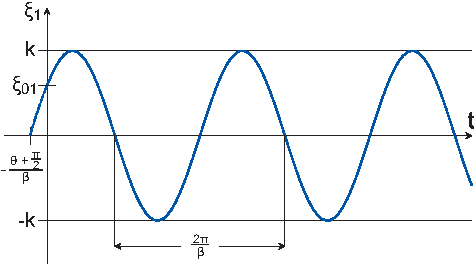
\includegraphics[width=0.4\textwidth]{img/Zustandsvariablen_Zeitverlauf1}

\subsubsection*{Schwach gedämpfte Schwingung (ZV2) $\lim_{t \to \infty} \xi_1(t)=0$}
Bei komplex konjugierten EW $\lambda_{1,2}=\alpha\pm j\beta;\;\;\;\;\alpha<0$\\\\
$\xi_1(t)=ke^{\alpha t}cos(\beta t+\Theta);\;\;\;\;\;\;\;\beta =\sqrt{{\omega_0}^2-\alpha^2};\;\;\;\alpha<0$\\\\
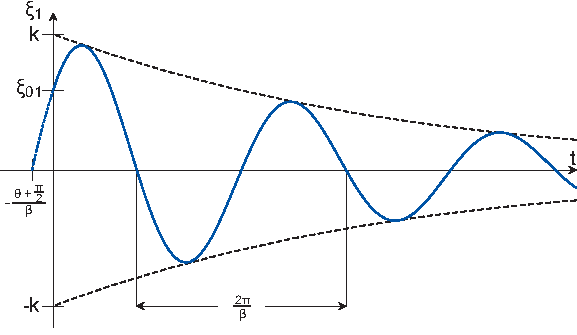
\includegraphics[width=0.4\textwidth]{img/Zustandsvariablen_Zeitverlauf2}

\subsubsection*{Stark gedämpfte Schwingung (ZV3)$\lim_{t \to \infty} \xi_1(t)=0$}
Bei rein reellen und unterschiedlichen Eigenwerten.\\\\
$\xi_1(t)=\xi_{01}e^{\lambda t};\;\;\;\;\;\;\lambda<0$\\\\
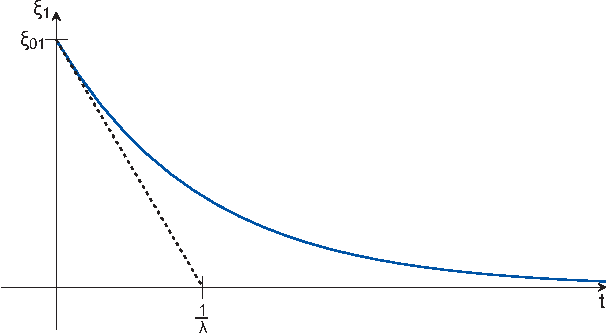
\includegraphics[width=0.4\textwidth]{img/Zustandsvariablen_Zeitverlauf3}\\\\
Da die Lösung für die Zustandsgrößen in der $\underline{x}$-Ebene eine Überlagerung von zwei Exponentialfunktionen ist, kann der Zeitverlauf dieser Zustandsgrößen jedoch Nulldurchgänge besitzen.

\subsubsection*{Aperiodisch gedämpfte Schwingung (ZV4)$\lim_{t \to \infty} \xi_1(t)=0$}
Falls beide Eigenwerte identisch sind.\\\\
$\xi_1(t)=(\xi_{01}+\xi_{02}t)e^{\lambda t};\;\;\;\;\;\;\lambda<0$\\\\
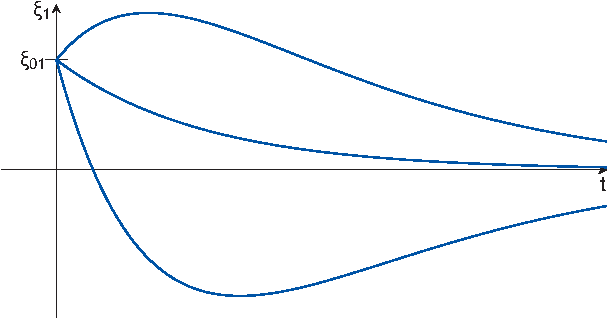
\includegraphics[width=0.4\textwidth]{img/Zustandsvariablen_Zeitverlauf4}\\\\

\section*{Nichtlineare dyn. Schaltungen}
\subsection*{1. Zustandsbeschreibung aufstellen}
Zustandsgröße:\\
Kapazität: $u_C$ (bzw. $q$); Induktivität: $i_L$ (bzw. $\Phi$)\\\\
$\dot{\underline{x}}=\left.\begin{matrix}\dot x_1 \\ \dot x_2\end{matrix}\right] =\underline{f}(\underline{x})=\left.\begin{matrix}f_1(x_1;x_2) \\ f_2(x_1;x_2)\end{matrix}\right]$\\\\
Zustandsgleichung mittels KCL, KVL, $i_c=C\dot u$ und $u_L=L\dot i$ aufstellen.\\\\
\subsection*{2. Alle Gleichgewichtspunkte bestimmen}
$\dot x_1 =\dot x_2\sollsein 0\Rightarrow$ nach $x_1$ und $x_2$ auflösen.\\\\
\underline{Alternativ:}\\
Direkt aus Schaltung bestimmen: $C\rightarrow$ LL; $L\rightarrow$ KS
\subsection*{3. Linearisierung in allen Gleichgewichtspunkten}
Jacobi-Matrix aufstellen: $\textbf{J}_{GGP_i}=\left.\begin{bmatrix}\frac{\partial f_1}{\partial x_1} & \frac{\partial f_1}{\partial x_2}\\ \frac{\partial f_2}{\partial x_1} & \frac{\partial f_2}{\partial x_2}\end{bmatrix}\right|_{\underline{x}=GGP_i}$\\\\
In $P_i=GGP_i$ linearisierte Beschreibung:\\\\
$\dot{\underline{x}}=\underline{f}(\underline{x})\approx \underline{f}(\underline{P}_i)+\textbf{J}_{\underline{P}_i}\cdot (\underline{x}-\underline{P}_i);\;\;\;\Delta \dot x\approx \textbf{J}_{\underline{P}_i}\Delta x$
\subsection*{4. Eigenwerte / Eigenvektoren bestimmen}
Für alle $\textbf{J}_{GGP_i}$ die Eigenwerte / Eigenvektoren bestimmen.\\\\
$\Rightarrow$ Phasenportrait in der Umgebung des GGP
\subsection*{5. Prüfen, ob Satz von Hartmann gilt}
Satz von Hartmann:\\
Linearisierung gültig $\Leftrightarrow \forall \lambda_i$ von $\textbf{J}_{GGP_i}$ gilt: $Re(\lambda_i)\neq 0$\\\\
Ist der Realteil eines Eigenwertes null, so kann man keine Aussage über das Stabilitätsverhalten treffen (Ausnahme: stückweise lineare Systeme)
\subsection*{6. Einzel-Phasenportraits zusammenfügen}
Wenn alle Bauelemente der Schaltung ungepolt sind, so ist das Phasenportrait punktsymmetrisch zum Ursprung.

\subsection*{Konservative Schaltungen}
(Jede verlustlose Schaltung ist konservativ, hinreichend genaue Modelle realer Schaltungen sind niemals konservativ!)\\\\
Bedingung: $\dot E=0;\;\;\;\;\;\frac{\partial E}{\partial x_1}f_1+\frac{\partial E}{\partial x_2}f_2=0$
\begin{enumerate}[label=-,leftmargin=3mm]
	\item nur Sattel- und Wirbelpunkte sind als Arten von Gleichgewichtspunkten möglich
	\item Trajektorien sind Äquipotentiallinien der Energiefunktion
\end{enumerate}
Gespeicherte Energie: $E=\frac{1}{2}(Cu_C^2+Li_L^2)$\\\\
Scheitelwerte: $\hat{u}_C=\sqrt{\frac{2E}{C}};\;\;\;\;\hat{i}_L=\sqrt{\frac{2E}{L}}$\\\\
Dauer eine Umlaufes: $T_0=2\pi \sqrt{LC}$\\\\
$u_C=\hat{u}_C cos(\omega t-\Phi_0);\;\;\;\;\;\;i_L=\hat{i}_L sin(\omega t-\Phi_0)$\\\\
Ergänzung zum Satz von Hartmann:\\
Ein GGP einer nichtlinearen dynamischen Schaltung ist genau dann ein Wirbelpunkt, wenn seine Jacobi-Matrix rein imaginäre Eigenwerte hat und das System in einer offenen Umgebung $U$ des GGP konservativ ist.

\subsection*{Oszillatoren}
Eine stabile Oszillation kann sich nur in einem nichtlinearen System einstellen.
\begin{enumerate}[label=-,leftmargin=3mm]
	\item Phasenportrait ist stabiler Grenzzyklus
	\item autonomes, dynamisches System zweiten Grades
	\item Es darf nur ein Gleichgewichtspunkt existieren und dieser muss instabil sein.
	\item Trajektorien müssen zu allen Anfangswerten aus Umgebung $U$ beschränkt sein
	\item Zustandsgrößen müssen beschränkt sein (bei positiven, linearen $C$, $L$ und $R$ immer der Fall)
\end{enumerate}
\subsubsection*{Fast harmonischer Oszillator}
\begin{enumerate}[label=-,leftmargin=3mm]
	\item Frequenz abhängig von den Werten der Reaktanzen
	\item Amplitude abhängig von Nichtlinearität der Bauteile
\end{enumerate}
Resonanzfrequenz: $\omega_0=\frac{1}{\sqrt{LC}}$
\subsubsection*{Relaxationsoszillator}
Frequenz und Amplitude werden wesentlich von Nichtlinearität der Bauteile bestimmt\\\\
$\omega_0=\frac{\pi}{ln(3)}\cdot \frac{1}{RC};\;\;\;2\sqrt{\frac{L}{C}}<<R$

\section*{Komplexe Wechselstromrechnung}
\subsection*{Voraussetzungen}
\begin{enumerate}[label=-,leftmargin=3mm]
	\item lineares, zeitinvariantes, stabiles System mit periodischer Erregung.
\end{enumerate}
Bei sinusförmiger Erregung mit der Kreisfrequenz $\omega$ sind alle Signale in der Schaltung sinusförmig mit der gleichen Kreisfrequenz.\\
Es entstehen keine neuen Frequenzen!
\subsection*{Zeigerdarstellung}
Zum reellen Signal $x(t)=A_m cos(\omega t+\alpha)$ wird der Zeiger $A=A_m e^{j\alpha}$ assoziiert. Mit der Amplitude $A_m$ und Phase $\alpha$.\\\\
Es gilt:\\
$x(t)=A_m cos(\omega t+\alpha)=Re(A_m e^{j(\omega t+\alpha)})$\\\\
$x(t)=Re(A_m e^{j\alpha}e^{j\omega t})=Re(Ae^{j\omega t})$\\\\
\begin{minipage}[t]{0.23\textwidth}
\subsubsection*{Kapazität}
$I_C=j\omega CU_C;\;\;U_C=\frac{1}{j\omega C}I_C$
\end{minipage}
\hfill
\begin{minipage}[t]{0.23\textwidth}
\subsubsection*{Induktivität}
$I_L=\frac{1}{j\omega L}U_L;\;\;U_L=j\omega LI_L$
\end{minipage}
\subsection*{Hilfssätze}
\subsubsection*{Lemma 1: Eindeutigkeit}
$a(t)=b(t)\Leftrightarrow A=B;\;\;\;\;$ Signale gleich $\Leftrightarrow$ Zeiger gleich
\subsubsection*{Lemma 2: Linearität}
$\alpha a(t)+\beta b(t)=c(t)\Leftrightarrow \alpha A+\beta B=C$
\subsubsection*{Lemma 3: Differentiation}
$b(t)=\frac{d}{dt}a(t)\Leftrightarrow B=j\omega A$
\subsection*{Netzwerkfunktionen}
\subsubsection*{Zweipolfunktionen}
= Verhältnis von Zeigern des gleichen Tores (Immittanzen)\\\\
\underline{Impedanz} (komplexer Widerstand, Scheinwiderstand):\\\\
$Z=\frac{U}{I};\;\;\;Z_G=\frac{1}{G};\;\;\;Z_L=j\omega L;\;\;\;Z_C=\frac{1}{j\omega C};\;\;\;Z=R+jX$\\\\
$Z$: Impedanz(Scheinkomponente)\\
$R$: Resistanz (Wirkkomponente)\\
$X$: Reaktanz (Blindkomponente)\\\\
\underline{Admittanz} (komplexer Leitwert, Scheinleitwert):\\\\
$Y=\frac{I}{U};\;\;\;Y_R=\frac{1}{R};\;\;\;Y_L=\frac{1}{j\omega L};\;\;\;Y_C=j\omega C;\;\;\;Y=G+jB$\\\\
$Y$: Admittanz (Scheinkomponente)\\
$G$: Konduktanz (Wirkkomponente)\\
$B$: Suszeptanz (Blindkomponente)
\subsubsection*{Übertragungfunktion}
= Verhältnis von Zeigern unterschiedlicher Tore\\\\
Allgemein: $H(j\omega)=\frac{OUTPUT}{INPUT}$\\\\
\underline{Knotenspannungsanalyse:}\\\\
$\underline{U}_K={\textbf{Y}_K}^{-1}(j\omega)\underline{I}_q;\;\;\;\;\;\;\underline{I}_q=(0,...,0,I_n,0,...0)^T$\\\\
$H(j\omega)=\frac{U_{Km}}{I_n}=\frac{(-1)^{n+m}det\textbf{Y}_{nm}(j\omega)}{det\textbf{Y}_K(j\omega)}$\\\\
$det\textbf{Y}_{nm}(j\omega)$ ist die Unterdeterminante von $\textbf{Y}_K$, die nach streichen der $n$-ten Zeile und $m$-ten Spalte entsteht.\\\\
\underline{Cramer'sche Regel:}\\\\
$U_{K_i}=\frac{det\textbf{Y}_{K_i}}{det\textbf{Y}_K}$\\\\
$det\textbf{Y}_{K_i}$ entsteht durch Ersetzen der $i$-ten Spalte in $\textbf{Y}_K$ durch $\underline{I}_q$\\\\
\underline{Eigenfrequenzen:}\\\\
Substitution $j\omega \rightarrow p$\\\\
Die Nullstellen des Nenner-Polynoms von $H(p)$ entsprechen genau den Eigenfrequenzen des Systems (sofern sie nicht durch Nullstellen des Zähler-Polynoms herauskürzbar sind)\\\\
Das System ist stabil, wenn der Realteil aller Nullstellen des Nenners $<0$ ist.
\subsection*{Darstellung des Frequenzgangs}
\subsubsection*{1. Ortskurve}
Die Ortskurve von $H(j\omega)$ ist die Kurve, die der komplexe Zeiger $H(j\omega)$ für $\omega =0$ bis $\omega \rightarrow \infty$ durchläuft.\\
Die Ortskurve ist die Zusammenfassung des Amplituden- und Phasenverlaufs des Bodediagramms.\\
Dabei ist die Frequenzabhängigkeit nur mehr über Markierungen auf der Kurve darstellbar.
\begin{enumerate}[leftmargin=3mm]
	\item Aufteilen von $H(j\omega)$ in $Re()$ und $Im()$
	\item Werte für $\omega =0, \omega =\omega_0$ (Resonanzfrequenz) und $\omega \rightarrow\infty$ bestimmen
	\item Komplexe Ebene: Punkte für einzelne Werte einzeichnen. Die Verbindungslinie entspricht der Ortkurve
\end{enumerate}
\underline{Anmerkung:}\\\\
Komplexer Widerstand $Z$ ist:
\begin{enumerate}[label=-,leftmargin=3mm]
	\item in Widerstandsebene: Gerade
	\item in Leitwertsebene: Kreis
\end{enumerate}
Komplexer Leitwert $Y$ ist:
\begin{enumerate}[label=-,leftmargin=3mm]
	\item in Widerstandsebene: Kreis
	\item in Leitwertsebene: Gerade
\end{enumerate}
\subsubsection*{2. Bode-Diagramm}
$v(\omega)=20lg\left|\frac{H(j\omega)}{H(j\omega_0)}\right| [dB];\;\;\;\;v(\omega)=ln\left|\frac{H(j\omega)}{H(j\omega_0)}\right| [Np]$\\\\
$1Np\entspr \frac{20}{ln(10)}dB\approx 8,686 dB;\;\;\;1dB\approx 0,115Np$\\\\
$\varphi(\omega)=\begin{cases}arctan\frac{Im(H(j\omega))}{Re(H(j\omega))} & Re(H(j\omega))\geq 0 \\arctan\frac{Im(H(j\omega))}{Re(H(j\omega))}+\pi & Re(H(j\omega))<0\end{cases}$\\\\
\underline{Rechenregeln:}\\\\
$v(H_1H_2)=v(H_1)+v(H_2);\;\;\;v(\frac{H_1}{H_2})=v(H_1)-v(H_2)$\\\\
$\varphi(H_1H_2)=\varphi(H_1)+\varphi(H_2);\;\;\;\varphi(\frac{H_1}{H_2})=\varphi(H_1)-\varphi(H_2)$\\\\
\underline{Beispiele:}\\\\
$H(j\omega)=k=konst.\;\;\Rightarrow v(\omega)=20lg|k|$\\\\
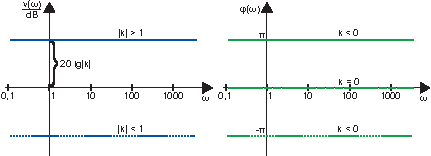
\includegraphics[width=0.48\textwidth]{img/Bode-Diagramm1}\\\\
$(1): H(j\omega)=\frac{j\omega}{\alpha};\;\;\;\;\;\;\;(2): H(j\omega)=\frac{\alpha}{j\omega}$\\\\
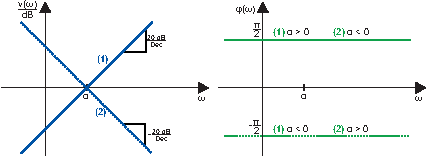
\includegraphics[width=0.48\textwidth]{img/Bode-Diagramm2}\\\\
$H(j\omega)=1+\frac{j\omega}{\alpha}$\\\\
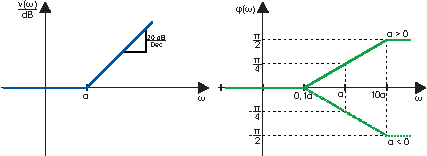
\includegraphics[width=0.48\textwidth]{img/Bode-Diagramm3}\\\\
$H(j\omega)=\frac{1}{1+\frac{j\omega}{\alpha}}$\\\\
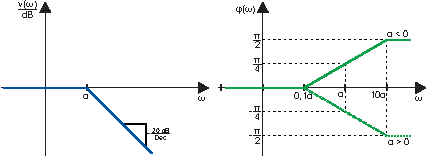
\includegraphics[width=0.48\textwidth]{img/Bode-Diagramm4}\\\\\\
\underline{Typische Übertragungsfunktionen:}\\\\
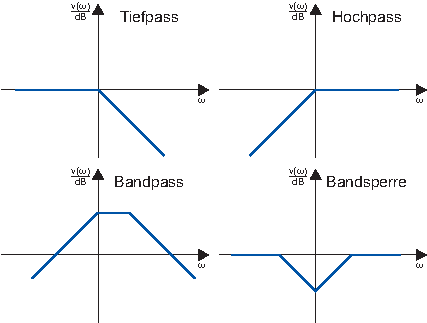
\includegraphics[width=0.48\textwidth]{img/Bode-Diagramm_typisch}\\
\subsection*{Komplexe Leistung}
Scheinleistung: $P_S=\frac{1}{2}\hat{U}\hat{I}^*=\frac{1}{2}|\hat{U}|^2Y^*=P_W+jP_B$\\\\
Wirkleistung: $P_W=\frac{1}{T}\cdot \int\limits_{0}^{T}u(t)i(t)dt=Re(P_S)$\\\\
Blindleistung: $P_B=Im(P_S)$
\subsection*{Sonstiges}
\subsubsection*{Resonanzfrequenz}
$\omega_0 =\frac{1}{\sqrt{LC}};\;\;\;f_0=\frac{1}{2\pi \sqrt{LC}}$
\subsubsection*{Grenzfrequenz (Grenzen der Bandbreite)}
$|Re(Y)|=|Im(Y)|;\;\;\;\;|Re(Z)|=|Im(Z)|$\\\\
$f_g=\frac{R}{2\pi L};\;\;\;\;f_g=\frac{1}{2\pi RC}$
\subsubsection*{Güte}
$Q=\frac{\omega_0 C}{G}=\frac{1}{\omega_0 LG}=\frac{1}{G}\sqrt{\frac{C}{L}}$
\\\\\\\\
Lizenz: CC BY-NC-SA 3.0\\
http://creativecommons.org/licenses/by-nc-sa/3.0/de/
\newpage
\begin{figure*}
\begin{center}
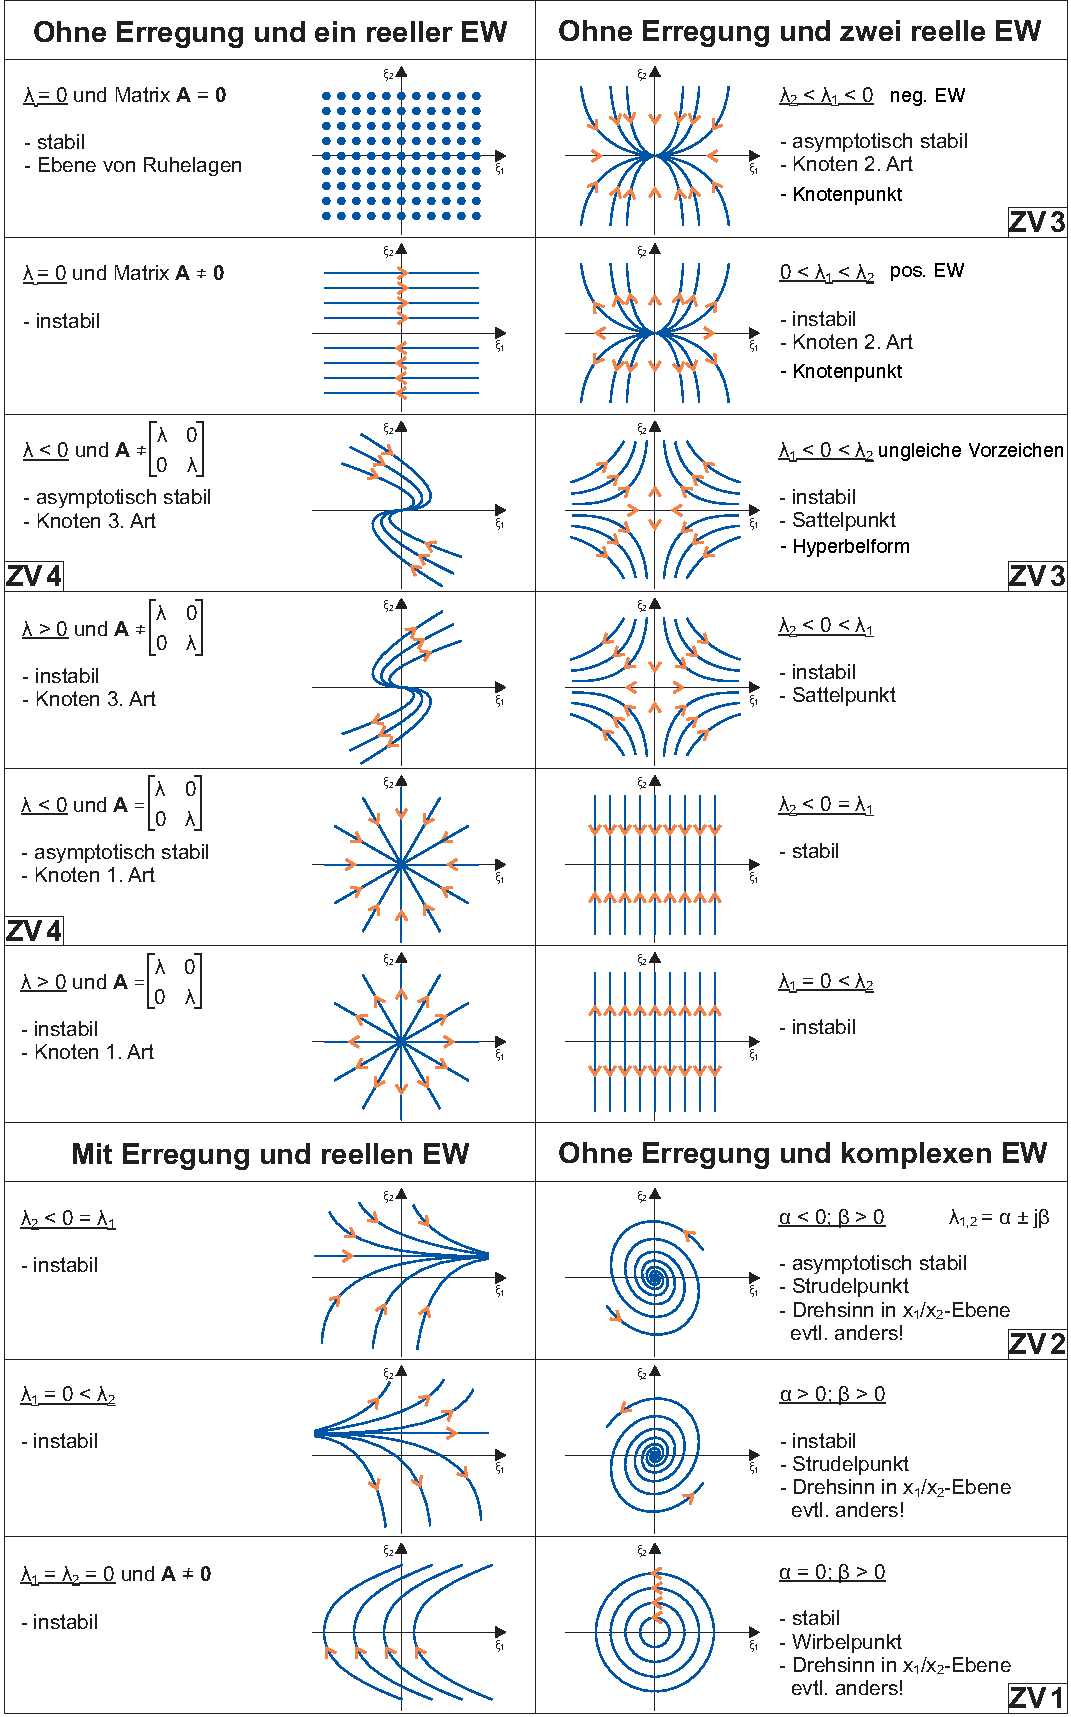
\includegraphics[width=0.85\textwidth]{img/Phasenportraits-annotated}
\end{center}
\end{figure*}

\end{document}
